\newcommand{\ttt}[1]{\texttt{#1}}

\section{Large Scale Structure}
Large scale structure studies require some important features: survey uniformity and optimized survey area that maximizes usable survey footprint with deep photometric data.  We discuss these features in the subsections below.
%%%%%%%%%%%%%%%%%%%%%%%%%%%%%%%%%%%%%%%%%%%%%%%%%%%%%%%%%%%%%%%%%%%%%%%%%%%%%%%%%%%%
\subsection{Survey Uniformity}
The effects of the LSST observing strategy on survey uniformity were explored extensively in \citet{Awan+2016}, with a follow-up in \citet[Section 9.2]{Marshall:2017wph}. The key result of these investigations is that frequent, large translational $dithers$ -- telescope-pointing offsets -- are critical to ensure survey uniformity, where $large$ is considered to be on the scale of the LSST FOV (1.75 deg). For the analyses here, we implement large, random offsets every night; note that while per night translational dithers are not the most frequent, dithering only once per night allows for maintaining the same systematics between visit-pairs and hence better calibrations. These dithers were implemented using the MAF Stacker, \href{https://github.com/lsst/sims_maf/blob/97988f6bc30c216fffb41e6da0a7d201e919b9ca/python/lsst/sims/maf/stackers/ditherStackers.py#L371}{RandomDitherPerNightStacker}; see more \href{https://github.com/LSSTDESC/ObsStrat/tree/issue/3/desc-dithers}{here}.

%%%%%%%%%%%%%%%%%%%%%%%%%%%%%%%%%%%%%%%%%%%%%%%%%%%%%%%%%%%%%%%%%%%%%%%%%%%%%%%%%%%%
\subsection{Optimized WFD Footprint}
Now, in order to select a galaxy sample for LSS studies, we must implement selection cuts. Specifically, to attain a Y10 gold sample at $i<25.3$, where $i$ is the $i$-band coadded 5$\sigma$ depth $after$ accounting for MW extinction, we must require a limiting 5$\sigma$ magnitude of $i=26.0$, alongside restricting to the region with E(B-V) $<0.2$ in order to minimize the systematics induced by the uncertainties in the dust map (need a reference). Furthermore, we focus on the footprint that has coverage in all six LSST filters in order to assure good photo-$z$ quality; for Y10, this comprises of $\sim$19,091 deg$^2$ in the current baseline, \ttt{baseline2018a}. Implementing our selection cuts (on coadded depth and extinction) reduces the usable footprint to $\sim$14,645 deg$^2$, hence discarding  $\sim$23\% of the WFD survey area. Figure~\ref{fig: skymaps_baseline_10yr} shows the skymaps before and after our selection cuts for the $i$-band coadded 5$\sigma$ depth after Y10.

%-------------------------------------------------------------------------------------
%-------------------------------------------------------------------------------------
\begin{figure}[H]
	\vspace*{2em}
	\centering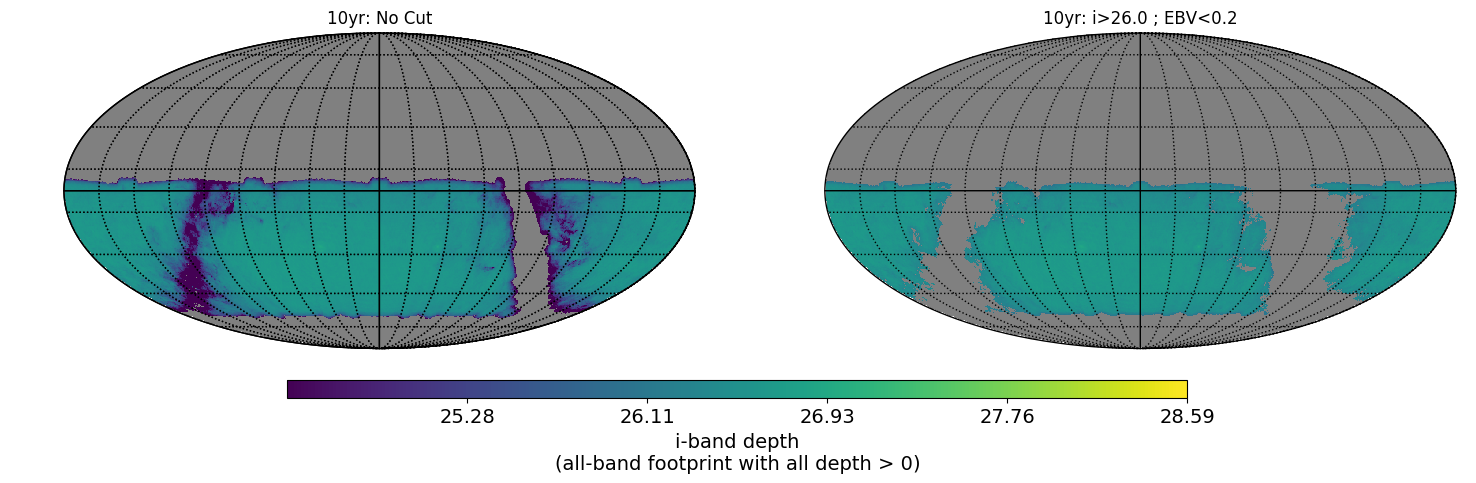
\includegraphics[width=\linewidth,trim={30 40 40 40},clip=false]{figures/lss_final_footprint_skymap_baseline2018a_nside256_RandomDitherPerNight_10yr_iband.png}
	\vspace*{1em}
	\caption{Skymaps for Y10  $i$-band coadded 5$\sigma$ depth for \ttt{baseline2018a}, limited to the footprint with coverage in all six bands, with random, per night translational dithers. \textit{Left}: Before any selection cuts.  \textit{Right}: After a depth cut of $i>26.0$ and an extinction cut of E(B-V)$<0.2$.}
	\label{fig: skymaps_baseline_10yr}
\end{figure}
%-------------------------------------------------------------------------------------

We find similar results when we implement selection cuts on Y1 data, now with a limiting 5$\sigma$ magnitude of $i=24.5$: the WFD footprint drops from $\sim$18,085 deg$^2$ to $\sim$13,613 deg$^2$, rendering $\sim$25\% of the nominal survey area unusable for our purposes.  Figure~\ref{fig: skymaps_baseline_1yr} shows the skymaps before and after our selection cuts for the $i$-band coadded 5$\sigma$  depth.

%-------------------------------------------------------------------------------------
%-------------------------------------------------------------------------------------
\begin{figure}[H]
	\vspace*{2em}
	\centering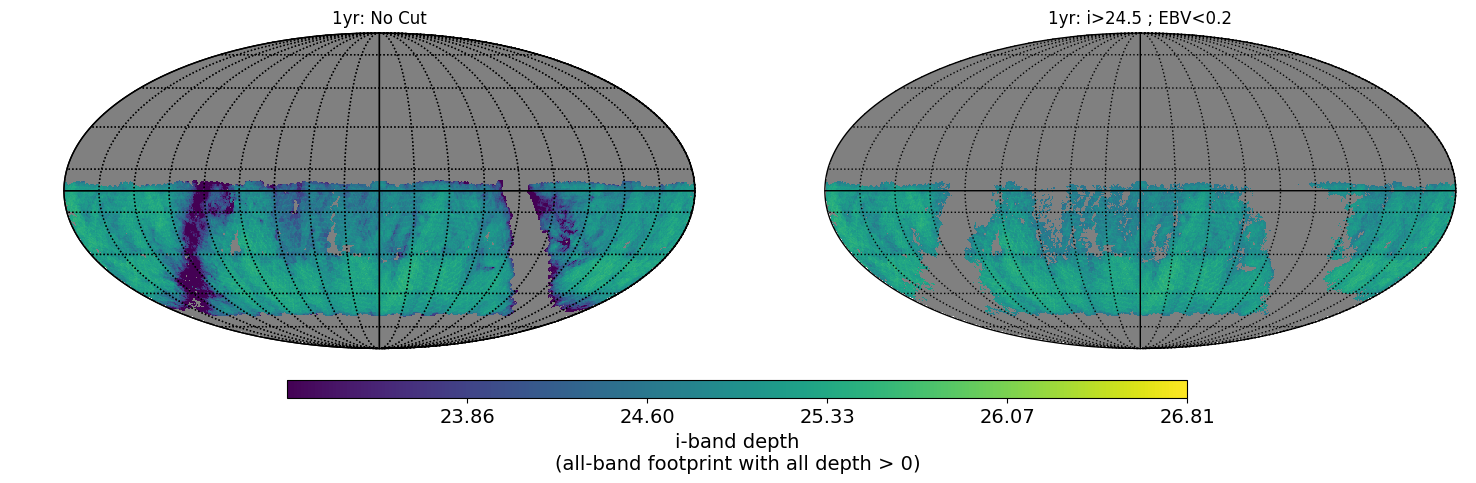
\includegraphics[width=\linewidth,trim={30 40 40 40},clip=false]{figures/lss_final_footprint_skymap_baseline2018a_nside256_RandomDitherPerNight_1yr_iband.png}
	\vspace*{1em}
	\caption{Skymaps for Y1 $i$-band coadded 5$\sigma$ depth for \ttt{baseline2018a}, limited to the footprint with coverage in all six bands with random, per night translational dithers. \textit{Left}: Before any selection cuts.  \textit{Right}: After a depth cut of $i>24.5$ and an extinction cut of $E(B-V)<0.2$.}
	\label{fig: skymaps_baseline_1yr}
\end{figure}
%-------------------------------------------------------------------------------------

In order to circumvent the issue of discarding a significant fraction of the WFD region, we propose a reconfiguration of the nominal WFD footprint to be limited to $only$ the footprint with E(B-V)$<0.2$, allowing for optimization of the WFD footprint that is usable for our science. To illustrate this, we consider the wider-coverage \ttt{OpSim} cadence, \ttt{pontus\_2002} and implement similar selection cuts as we did for \ttt{baseline2018a}. For Y1, the final footprint consists of $\sim$15,544 deg$^2$ while Y10 footprint comprises $\sim$19,254 deg$^2$, illustrating that the WFD footprint $can$ be optimized to yield large extragalactic footprint; Figures~\ref{fig: skymaps_pontus2002_10yr}-\ref{fig: skymaps_pontus2002_1yr}  show the analogs of Figures~\ref{fig: skymaps_baseline_10yr}-\ref{fig: skymaps_baseline_1yr} for \ttt{pontus\_2002}.

%-------------------------------------------------------------------------------------
%-------------------------------------------------------------------------------------
\begin{figure}[H]
	\vspace*{2em}
	\centering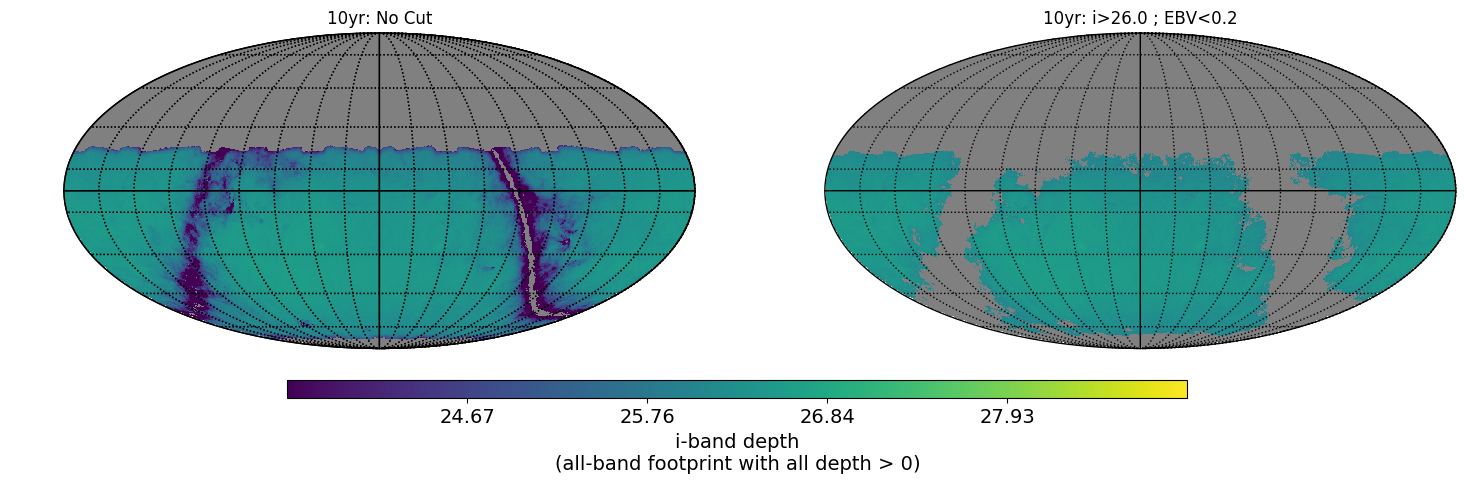
\includegraphics[width=\linewidth,trim={30 40 40 40},clip=false]{figures/lss_final_footprint_skymap_pontus_2002_nside256_RandomDitherPerNight_10yr_iband.png}
	\vspace*{1em}
	\caption{Skymaps for Y10 $i$-band coadded 5$\sigma$ depth for \ttt{pontus\_2002}, limited to the footprint with coverage in all six bands with random, per night translational dithers. \textit{Left}: Before any selection cuts.  \textit{Right}: After a depth cut of $i>26.0$ and an extinction cut of E(B-V)$<0.2$.}
	\label{fig: skymaps_pontus2002_10yr}
\end{figure}
%-------------------------------------------------------------------------------------
%-------------------------------------------------------------------------------------
%-------------------------------------------------------------------------------------
\begin{figure}[H]
	\vspace*{2em}
	\centering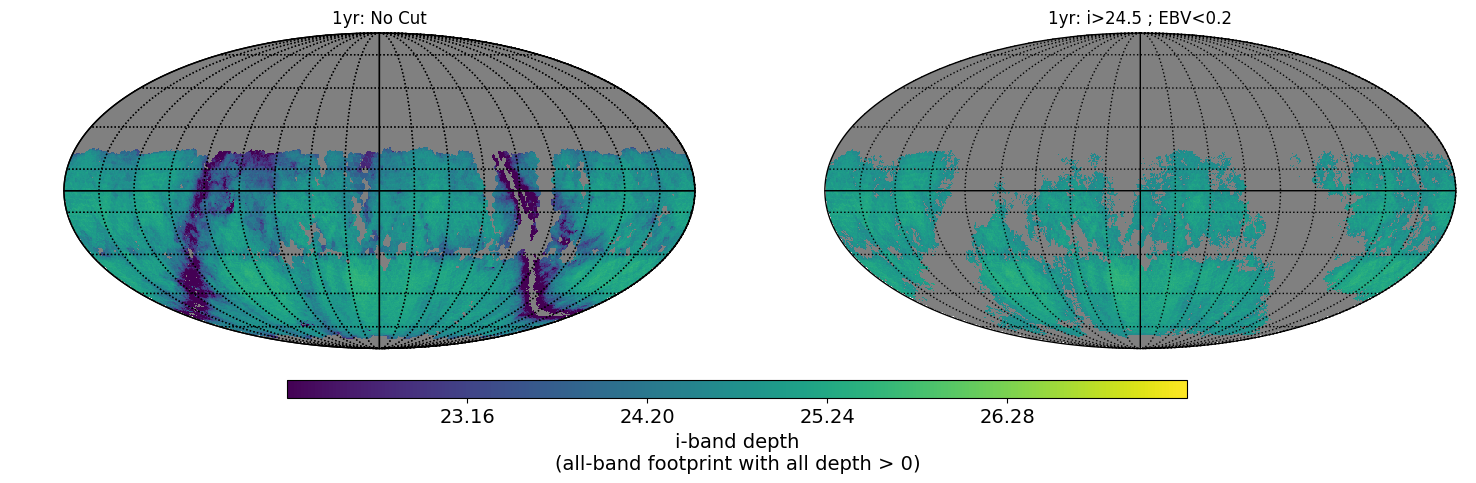
\includegraphics[width=\linewidth,trim={30 40 40 40},clip=false]{figures/lss_final_footprint_skymap_pontus_2002_nside256_RandomDitherPerNight_1yr_iband.png}
	\vspace*{1em}
	\caption{Skymaps for Y1  $i$-band coadded 5$\sigma$ depth for \ttt{pontus\_2002}, limited to the footprint with coverage in all six bands with random, per night translational dithers. \textit{Left}: Before any selection cuts.  \textit{Right}: After a depth cut of $i>24.5$ and an extinction cut of $E(B-V)<0.2$.}
	\label{fig: skymaps_pontus2002_1yr}
\end{figure}
%-------------------------------------------------------------------------------------
 Keeping these concerns in mind, we have requested a full \ttt{OpSim} run restricted to the footprint with E(B-V)$<0.2$; please see \href{https://github.com/LSSTDESC/ObsStrat/tree/issue/5/modify-wfd}{here} for more details. We are awaiting the \ttt{OpSim} output in order to assess the depth and uniformity coverage achievable in the reconfigured WFD survey area.

%%%%%%%%%%%%%%%%%%%%%%%%%%%%%%%%%%%%%%%%%%%%%%%%%%%%%%%%%%%%%%%%%%%%%%%%%%%%%%%%%%%%
\subsection{Extragalactic Footprint: Comparisons}
In order to compare the various cadences, we implement depth and extinctions cuts for four benchmarks in the ten-year survey: Y1, Y3, Y6, Y10, maintaining $i>24.5$ and $i>26.0$ cuts for Y1, Y10 respectively and extrapolating in between (hence $i>25.0$  for Y3 and $i>25.5$ for Y6). We compare the usable extragalactic footprint alongside the median $i$-band coadded 5$\sigma$ depth (to capture the achieved depth) and the standard deviation in the $i$-band coadded 5$\sigma$ depth (to capture the survey uniformity).

Figure~\ref{fig: compare_area} shows the footprint area for the four benchmarks for 17 different cadences. These include the baseline cadence, \ttt{baseline2018a}, the ten that are included in the WP call, and four new cadences (\ttt{kraken\_2042}, \ttt{kraken\_2044}, \ttt{mothra\_2049}, \ttt{nexus\_2097}); all these are translationally dithered post-\ttt{OpSim} simulation. We also consider five outputs from the feature-based scheduler (\ttt{cadence\_roll\_75\_mix}, \ttt{roll\_mix\_100}, \ttt{roll\_mix}, \ttt{rolling\_10yrs}, \ttt{tms\_roll\_10yrs}) and two \ttt{alt\_sched} outputs (\ttt{alt\_sched}, \ttt{alt\_sched\_rolling}); these do not need to be translationally dithered since translational dithering is built into the respective schedulers.

%-------------------------------------------------------------------------------------       
%-------------------------------------------------------------------------------------
\begin{figure}[H]
	\vspace*{2em}
	\centering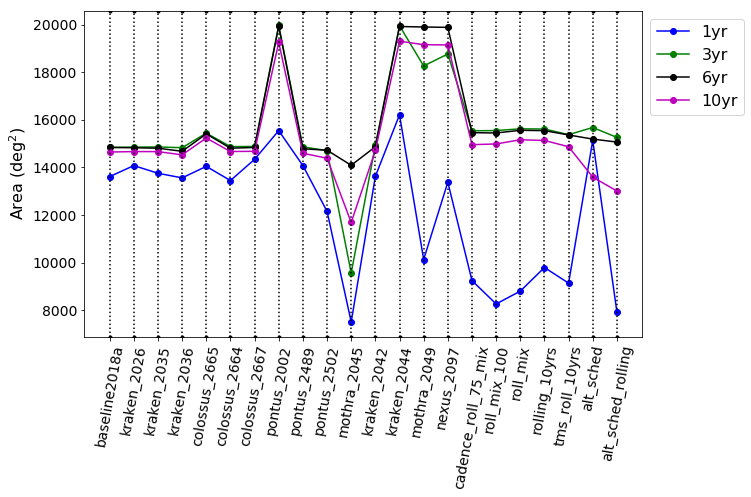
\includegraphics[width=0.5\paperwidth,trim={30 40 40 40},clip=false]{figures/lss_compare_area_22dbs.png}
	\vspace*{1em}
	\caption{Comparison of the usable survey area, following depth cuts ($i>24.5$ for Y1, $i>25.0$ for Y3, $i>25.5$ for Y6, $i>26.0$ for Y10) and an extinction cut (E(B-V)$<0.2$) for different cadences.}
	\label{fig: compare_area}
\end{figure}
%-------------------------------------------------------------------------------------

We see that for Y3, Y6, Y10, the cadences can loosely be grouped into three categories: 1) \ttt{pontus\_2002}, \ttt{kraken\_2044}, \ttt{mothra\_2049}, \ttt{nexus\_2097}, all of which yield significantly large usable footprint, 2) \ttt{mothra\_2045} which performs significantly unfavorably, and 3) the rest, leading to comparable final survey area.  All four cadences in the first category simulate very large WFD region (24,700 deg$^2$); \ttt{kraken\_2044} implements single visits per night, while \ttt{mothra\_2049} and \ttt{nexus\_2097} simulate different rolling cadences. On the other hand, \ttt{mothra\_2045} implements the same rolling cadences as  \ttt{mothra\_2049} but restricts to the nominal WFD region, leading to very limited survey footprint. Based on these comparison, we conclude that the larger WFD footprint, even with rolling cadence, is critical for our science.

As for Y1, the categorization is comparatively difficult.  \ttt{pontus\_2002}, \ttt{kraken\_2044} and \ttt{alt\_sched} yield the most area while all the outputs from the feature-based scheduler and the rolling  \ttt{alt\_sched} output perform as poorly as \ttt{mothra\_2045}. One notable takeaway is that specifics of the rolling cadence are critical for Y1, as we see, e.g., that $\sim$3,000 deg$^2$ is lost between the large WFD footprint with rolling cadence in 3 declination bands vs. 2 (i.e., \ttt{nexus\_2097} vs. \ttt{mothra\_2049}).

To compare the depth and its uniformity, Figure~\ref{fig: compare_depth} shows the median (left) and the standard deviation (right) for the $i$-band coadded 5$\sigma$ depth for the 17 cadences. We observe that the cadences achieve comparable median depths, with interesting trends across the benchmarks  (e.g., \ttt{mothra\_2045} leads to deepest Y1, Y3 but shallower Y6). The uniformity is more interesting, with \ttt{mothra\_2045} significantly more non-uniform than the rest of the cadences. We note that rolling in large WFD region leads to larger standard deviation than non-rolling, implying (again) the need to carefully select the rolling cadence specifics to be catered the LSST data releases.

%-------------------------------------------------------------------------------------
%-------------------------------------------------------------------------------------
\begin{figure}[H]
	\vspace*{2em}
	\begin{minipage}{.4\paperwidth}
		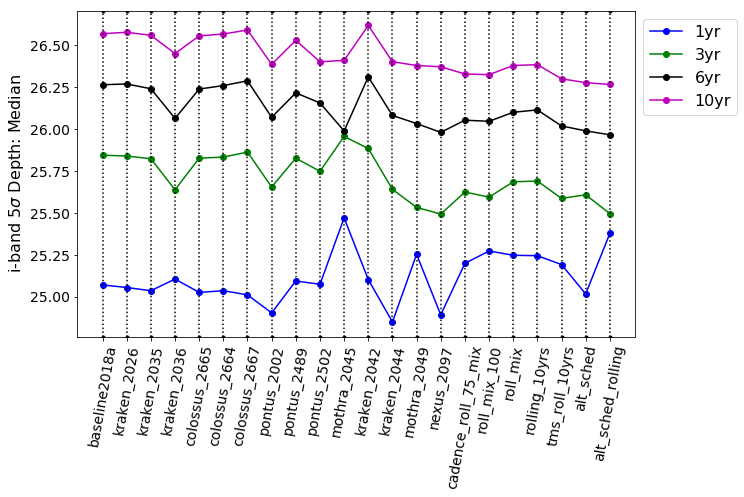
\includegraphics[width=.42\paperwidth, trim={5 20 100 10},clip=true]{figures/lss_compare_depth_median_22dbs.png}
	\end{minipage}\
	\hspace*{1em}
	\begin{minipage}{.4\paperwidth}
		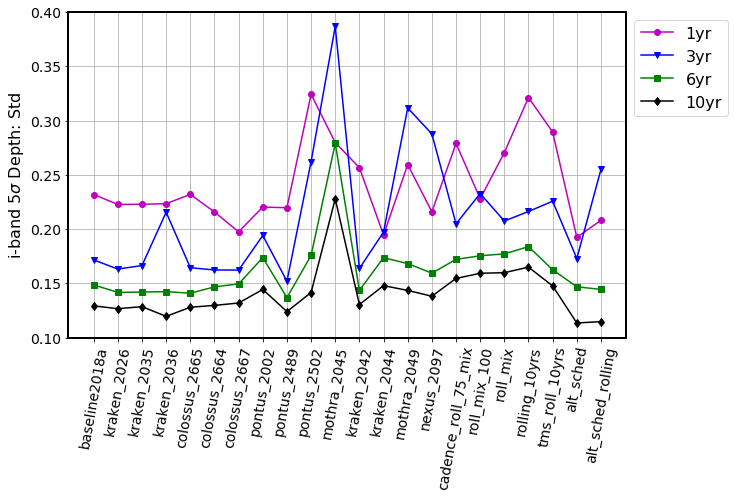
\includegraphics[width=.42\paperwidth, trim={5 20 80 10},clip=false]{figures/lss_compare_depth_std_22dbs.png}
	\end{minipage}
	\vspace*{1em}
	\caption{Comparison of two statistics on the $i$-band coadded 5$\sigma$ depth, following depth cuts ($i>24.5$ for Y1, $i>25.0$ for Y3, $i>25.5$ for Y6, $i>26.0$ for Y10) and an extinction cut (E(B-V)$<0.2$) for different cadences. \textit{Left}: Median depth. \textit{Right}: Standard deviation in the depth.}
\label{fig: compare_depth}
\end{figure}
%-------------------------------------------------------------------------------------

For exact numbers for the usable here and the depth statics, please see \href{https://github.com/LSSTDESC/ObsStrat/tree/static/static}{here}. More details about the implementation of the selection cuts are \href{https://github.com/LSSTDESC/ObsStrat/tree/static/static/depth\_cuts}{here}.

%%%%%%%%%%%%%%%%%%%%%%%%%%%%%%%%%%%%%%%%%%%%%%%%%%%%%%%%%%%%%%%%%%%%%%%%%%%%%%%%%%%%
\subsection{To Dos for LSS}
\enumerate{
\item Currently working on confirming that the OS systematics discussed in \citet{Awan+2016} are subdominant. Should be done in a few days.
\item Waiting on the \ttt{OpSim} output for the optimized WFD footprint to see how the depth changes once we have restricted to the optimized WFD footprint.
\item Translational dithering currently leads to shallower survey edges, given that the dithered pointings sometimes lead to partial coverage outside the nominal footprint. A solution to this issue is an "annealed" dither pattern, which preferentially doesn't dither outside a defined survey region. This might not be something to worry about if the feature-based scheduler is adopted as the official scheduler as there would be no need to dither post-\ttt{Opsim} simulation.
}

%%%%%%%%%%%%%%%%%%%%%%%%%%%%%%%%%%%%%%%%%%%%%%%%%%%%%%%%%%%%%%%%%%%%%%%%%%%%%%%%%%%%
\subsection{To Dos: Miscellaneous}
\enumerate{
\item Need to figure out a cleverer rotational dither strategy, at least ensuring no rotational dithers are implemented in between visit-pairs.
}

 
